\documentclass[12pt]{article}
\usepackage{graphicx, amsmath}
\usepackage{caption}
\graphicspath{ {./} }
\setlength{\oddsidemargin}{0.25 in}
\setlength{\evensidemargin}{-0.25 in}
\setlength{\topmargin}{-0.6 in}
\setlength{\textwidth}{6.5 in}
\setlength{\textheight}{8.5 in}
\setlength{\headsep}{0.75 in}
\setlength{\parindent}{0 in}
\setlength{\parskip}{0.1 in}

\begin{document}
\thispagestyle{plain}
   \newpage
   \setcounter{page}{1}
   \noindent
   \begin{center}
   \framebox{
      \vbox{\vspace{2mm}
    \hbox to 6.28in { {\bf BioE 131: Intro to Computational Biology}
                        \hfill Fall 2020 }
       \vspace{4mm}
       \hbox to 6.28in { {\bf \Large \hfill Multiple Alignment  \hfill} }
       \vspace{2mm}
       \hbox to 6.28in { {\it Professor: Ian Holmes \hfill} }
      \vspace{2mm}}
   }
   \end{center}
   {Notes written by Vikram Shivakumar}
   \vspace*{4mm}


\section{Introduction}
In the last note, we discussed pairwise alignment, aligning two sequences together by resolving gaps and substitutions using a few dynamic programming algorithms. However, often we would like to align \textit{more than two} sequences together! For example, we have sequenced a particular gene from 10 species in the \textit{Citrus} family, and we want to build an alignment of all 10 sequences so we can construct a phylogeny of the species based on this gene. In this note, we'll see that the dynamic programming algorithms from pairwise alignment are computationally expensive for tasks like these, but we will explore a few ways of approximating the \textbf{multiple alignments (MSA)}.

\section{Why not use Dynamic Programming?}
Dynamic Programming is often the efficient solution to many problems, many times yielding a polynomial runtime complextiy (i.e. $O(N^2)$ or $(O(N^3))$). In the case of a pairwise alignment, in all the DP algorithms we have covered, the runtime complexity is $O(L^2)$, where $L$ is the length of the two sequences. But what if we want to align three sequences together?\\[10pt]
Now, instead of a 2D DP matrix with one sequence on each axis, we will need a 3D matrix to include all three sequences of interest! Naturally the memory and runtime complexity of the alignment algorithm becomes $O(L^3)$, since there are now $L^3$ cells to calculate and store in the DP matrix. We can then generalize this to $N$ sequences of length $L$, where the runtime and memory complexity of a DP algorithm becomes $O(L^N)$.\\[10pt]
\begin{figure}[h]
    \centering
    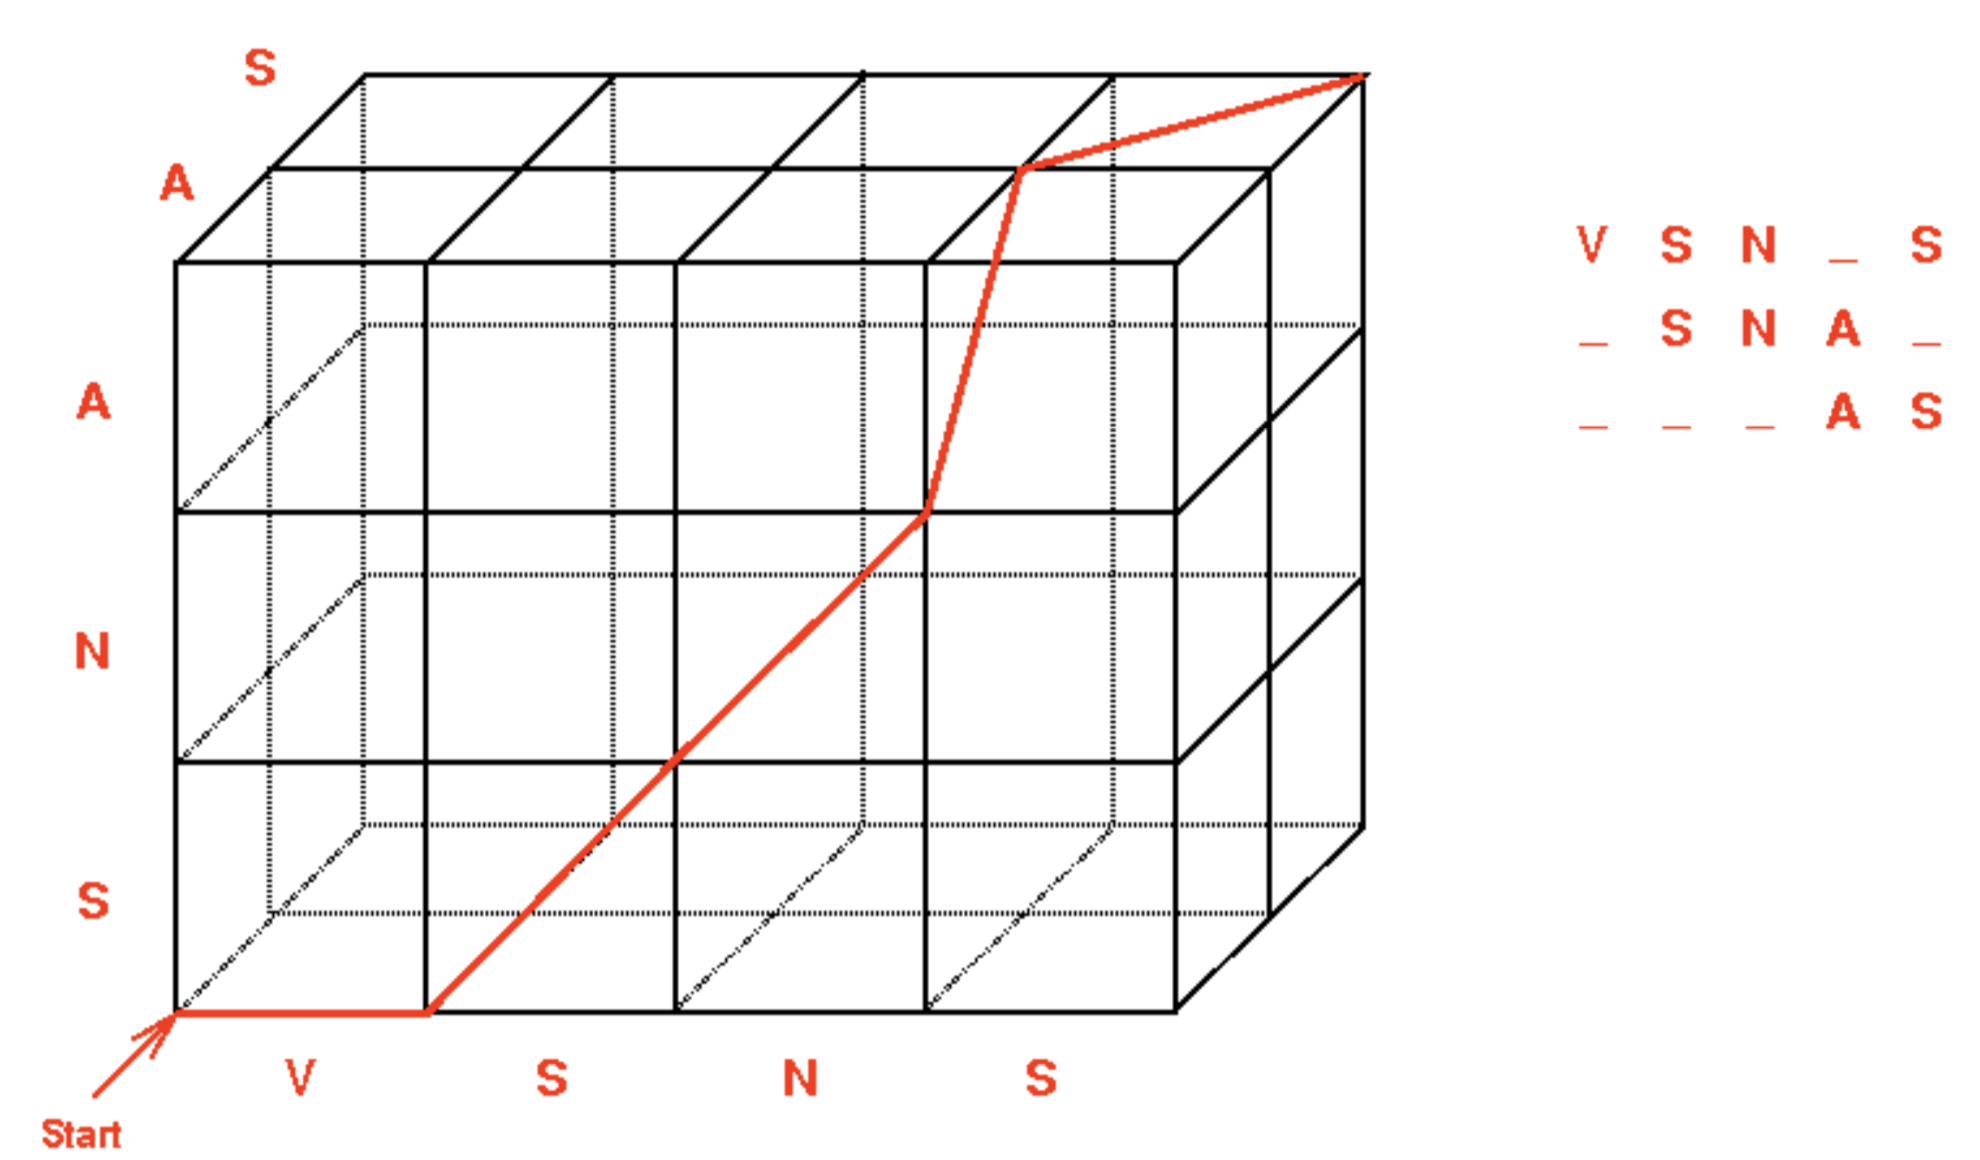
\includegraphics[width = .6\linewidth]{3d_dp.png}
    \caption{Example of a 3D Dynamic Programming Matrix}
    \label{fig:3d_dp}
\end{figure}
To understand why a runtime of $O(L^N)$ is infeasible, let's look at our example of aligning 10 genes. Assuming each gene is 200bp, and each cell in the DP matrix stores a floating point number (4 bytes), then the required space in memory for the algorithm to run would be $4 * (200^10) = 409,600 \text{ Exabytes}$, or around 409 trillion gigabytes. Even aligning just 5 of these sequences takes over 1000 GB. Thus we need a more efficient method for aligning multiple sequences!

\section{Progressive Alignment}
\subsection{Algorithm}
One method to efficiently construct a multiple alignment is the \textbf{progressive alignment} algorithm. This method approximates the full multiple alignment by iteratively aligning related sequences first, rather than aligning all the sequences at once. This involves a few steps before aligning:
\begin{enumerate}
    \item Pairwise align each sequence to every other sequence, and build a \textbf{distance matrix} for the sequences
    \item Build a \textbf{guide tree} from this distance matrix
    \item Build a \textbf{profile} for each internal node of the tree
    \item Starting from the leaves, \textbf{align siblings} together until all sequences are included
\end{enumerate}
\begin{figure}[h]
    \centering
    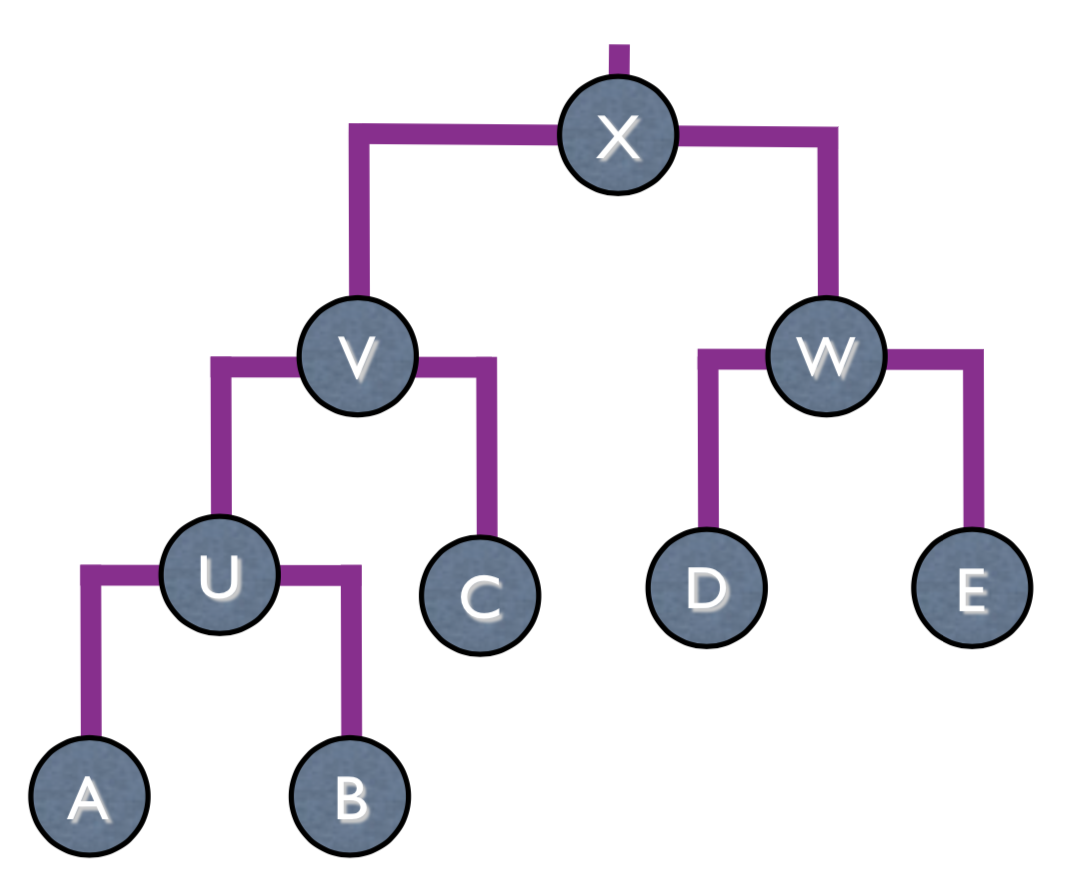
\includegraphics[width = .5\linewidth]{tree.png}
    \caption{Example guide tree for a progressive alignment of 5 sequences}
    \label{fig:tree}
\end{figure}
\subsection{Time/Memory Complexity}
The runtime complexity of the first step is $O(N^2L^2)$, since there are $(O(N^2))$ pairwise alignments, each taking $O(L^2)$ time (using any of the DP algorithms for pairwise alignment). Building a tree from the calculated distance matrix takes $O(N^3)$ time (see the note on Phylogenies for a detailed explanation). Building a profile for each internal node takes $O(NL^2)$, since there are $N-1$ internal nodes. Compared to the $O(L^N)$ runtime of a full DP algorithm, the progressive alignment is much more efficient.\\[10pt]
However, this alignment method serves as an \textit{approximation} of the full multi-dimensional DP alignment, and will not always converge to the optimal multiple alignment (which a full DP algorithm will always find). One reason is that final multiple alignment is dependent on the order of progressive alignment, where errors in early alignments are propagated through the iterative process. The final alignment can serve as a lower bound for the actual solution though, and can be improved using various techniques for \textbf{iterative refinement}.

\subsection{Sequence Profiles}
For the internal nodes in the guide tree, we need to build a \textbf{sequence profile}, which is a probabilistic model which describes a sequence motif. We can represent this model as a \textbf{Position Weight Matrix (PWM)}, which stores the probability of each nucleotide (or amino acid) at each position.
\begin{table}[h]
\centering
\begin{tabular}{r|rrrrrr}
A & .8 & 0  & .4 & .2 & 1 & 0   \\ \cline{2-7} 
C & 0  & .6 & .2 & .2 & 0 & 0   \\ \cline{2-7} 
G & 0  & 0  & .4 & .4 & 0 & .2 \\ \cline{2-7} 
T & .2 & .4 & 0  & .2 & 0 & .8
\end{tabular}
\caption{Example of a Position Weight Matrix}
\label{tab:pwm}
\end{table}
A PWM can generate sequences by randomly sampling a residue at each position from the probability distribution in each column. We can also determine the probability $P(X | \theta)$ that a sequence $X$ was generated by a PWN $\theta$:
$$\prod_{i\in X} q_i(X_i)$$
where $q_i(X_i)$ is the probability of residue $X_i$ at column $i$, which is given in the PWM. For example, the probability of the sequence ACAAAT would be $.8 * .6 * .4 * .2 * 1 * .8 \approx .03$\\[10pt]
If we assume a \textit{null} model, for example a uniform distribution at every position, than we can also calculate the posterior probability $P(\theta | X)$, e.g. the probability that that the sequence $X$ was produced by the model $\theta$, using Bayes Theorem (see the note on Probability).\\[10pt]
\begin{figure}[t]
    \centering
    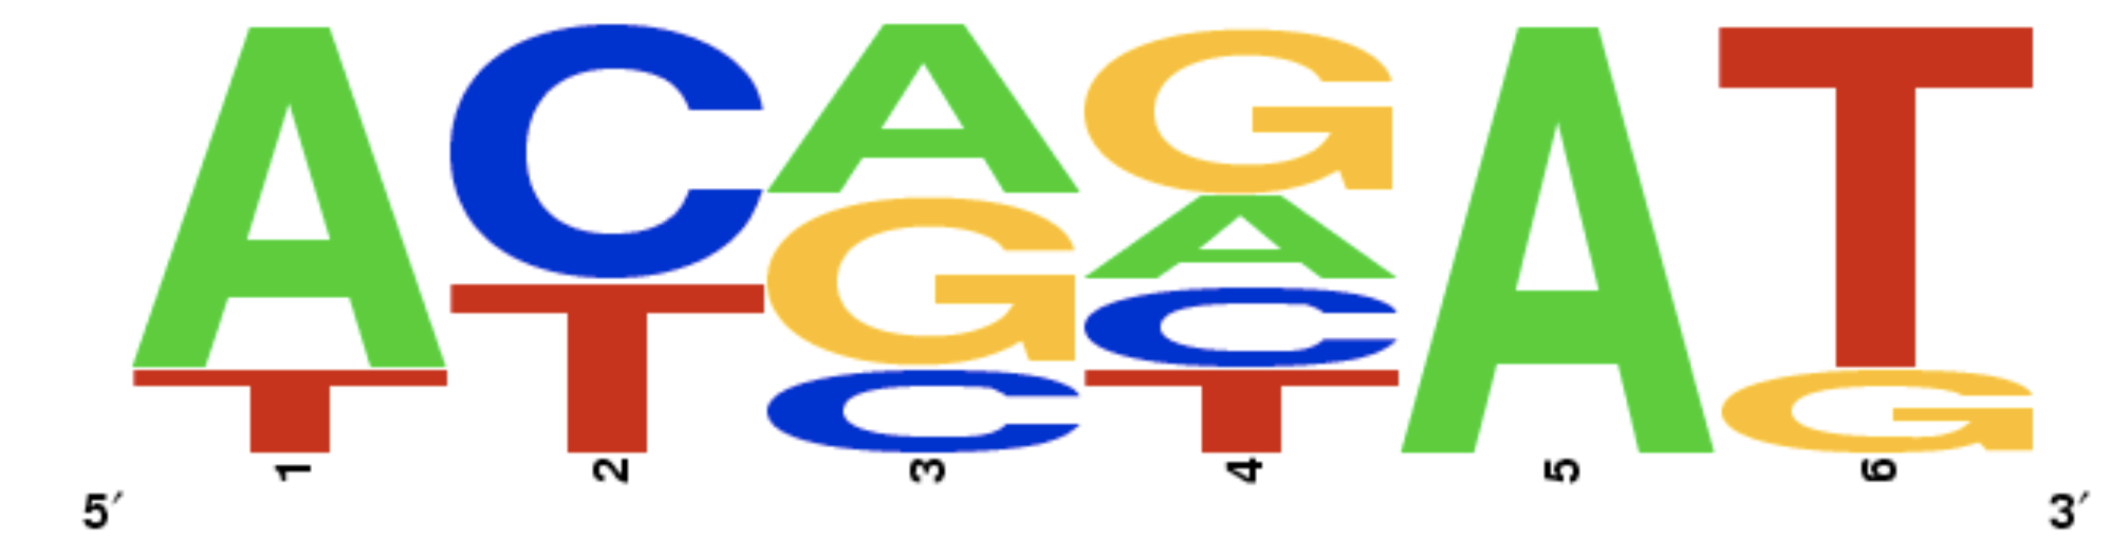
\includegraphics[width=.6\linewidth]{logo.png}
    \caption{Sequence logo of PWM in Table \ref{tab:pwm}}
    \label{fig:log}
\end{figure}
We can build a PWM from the columns of the alignment by counting the frequency of each nucleotide at each position and normalizing to get a probability distribution for each column. What if a nucleotide has a frequency of 0? Then when we calculate the likelihood of a sequence with that particular nucleotide at that position, $q_i(X_i) = 0$, and the above product is 0! Thus we need to introduce \textbf{Laplace pseudocounts}. Now when calculating the frequencies of each nucleotide, we add 1 to each value in the frequency table. For example, we can include pseudocounts for the PWM above:
\begin{table}[h]
\parbox{.45\linewidth}{
\centering
\begin{tabular}{r|rrrrrr}
A & 4/5 & 0  & 2/5 & 1/5 & 1 & 0   \\ \cline{2-7} 
C & 0  & 3/5 & 1/5 & 1/5 & 0 & 0   \\ \cline{2-7} 
G & 0  & 0  & 2/5 & 2/5 & 0 & 1/5 \\ \cline{2-7} 
T & 1/5 & 2/5 & 0  & 1/5 & 0 & 4/5
\end{tabular}
\caption*{Before pseudocounts}
}
\parbox{.45\linewidth}{
\centering
\begin{tabular}{r|rrrrrr}
A & 5/9 & 1/9  & 3/9 & 2/9 & 6/9 & 1/9   \\ \cline{2-7} 
C & 1/9  & 4/9 & 2/9 & 2/9 & 1/9 & 1/9   \\ \cline{2-7} 
G & 1/9  & 1/9  & 3/9 & 3/9 & 1/9 & 2/9 \\ \cline{2-7} 
T & 2/9 & 3/9 & 1/9  & 2/9 & 1/9 & 5/9
\end{tabular}
\caption*{After adding pseudocounts}
}
\end{table}
\section{Scoring Schemes}
\subsection{Column Scores}
Similar to pairwise alignments, there are various scoring schemes for multiple alignments. These schemes can be used to compare and evaluated a multiple alignment from an algorithm like progressive alignment to a \textbf{gold-standard}, often a structural alignment.\\[10pt]
One metric that is commonly used is the \textbf{Sum of Pairs Score (SPS)}, which evaluates a single column in an MSA. The SPS metric takes the sum of the substitution score over every combination of sequences:
$$S = \sum_i\sum_{j>i}Q(x_i, x_j)$$
where $Q(x_i, x_j)$ is the substitution score (from a BLOSUM matrix for example), and $x_i$ is the residue for the column for sequence $i$. One issue with the SPS score is that over-represented clades in a tree tend to dominate. The reason for this is every pair of sequences is compared, so if many sequences are similar and froma. single clade, the they would comprise the majority of the SPS score. Another metric is the \textbf{Total Column Score (TCS)}, which counts the number of columns in the MSA which are completely accurate. 

\subsection{Consensus Alignment}
Consensus alignments combine multiple alignments from different algorithms (progressive alignment, structural alignment, etc.) to form a final MSA. Some methods for consensus multiple alignment involve calculating the \textbf{posterior probability} of each residue pair. These methods are similar to the McCaskill algorithm from RNA folding, in that they compute a partition function over an ensemble of multiple alignments, and calculate the probability of a pair of residues by looking at all MSAs which include that pair of residues (similar to a partition function over an ensemble of RNA structures, and the probability of two bases being paired).\\[10pt]
Once the posterior probabilities are calculated, some algorithms use \textbf{expectation maximization} to maximize the SPS score over the MSA. Others find the closest related residues and start aligning those first (called \textbf{sequence annealing}). Lastly, some algorithms use these posterior probabilities to avoid comparing all $N^2$ sequence pairs, instead only making $O(N\log N)$ comparisons to ensure that the MSA contains all the sequences and is connected.


\section{Other Alignment methods}
Progressive alignments are used widely in various bioinformatic tools (CLUSTAL, MUSCLE, MAFFT), as are consensus methods (ProbCons, FSA). Aside from these methods, there are also structural alignment methods, which align proteins using 3D structure. Often these methods minimize the \textbf{root-mean-squared deviation (RMSD)} between two structures to determine the optimal alignment. Other algorithms are used to align RNA while simultaneously folding the RNA sequences (DynAlign, StemLoc, LocaRNA). Lastly, there are tools for aligning whole genomes and sequences with large rearrangements like bacterial/viral genomes (MAUVE, MAVID).

\section{Summary}
Often times computing the optimal alignment using dynammic programming can be infeasible, so several alignment approaches have been developed that use heuristics to direct alignment. For example progressive alignment uses the relationship between sequences to efficiently build the MSA. These tools allow us to study phylogenies and sequence relationships, as well as build sequence motif profiles as probabilistic models.


\end{document}


%topics not covered:
%why SPS allows some clades to dominate
%PWM entropy (proof for just normalizing frequencies?)
%TKF91 model, phylogenetic scores (maybe in the next module?), Phylogenetic automata
%Posterior prob